\documentclass[11pt]{amsart}

%\usepackage[notref,notcite]{showkeys}
\usepackage[style=authoryear,ibidtracker=false,uniquename=false,giveninits=true,terseinits=true,maxbibnames=5,backend=biber]{biblatex}
\usepackage{float}
\usepackage{graphicx}
\usepackage{todonotes}
\usepackage{subcaption}
\usepackage{amsmath}
\usepackage{amsthm}
\usepackage{amssymb}
\usepackage{algorithm}
\usepackage[noend]{algorithmic}
\usepackage[foot]{amsaddr}
\usepackage[misc]{ifsym}
\usepackage{enumitem}
\usepackage{geometry}
\usepackage[hidelinks]{hyperref}

%FOCS margins
\setlist{leftmargin = 0pt, labelindent = 0pt}
\geometry{margin=1in}

\renewbibmacro{in:}{}
\addbibresource{rnni_polynomial.bib}

\newtheorem{proposition}{Proposition}
\newtheorem{theorem}{Theorem}
\newtheorem{corollary}{Corollary}
\newtheorem{decision_problem}{Decision Problem}
\newtheorem{question}{Question}

\newcommand{\rnni}{\mathrm{RNNI}}
\newcommand{\findpath}{\textsc{FindPath}}
\newcommand{\mrca}{\mathrm{mrca}}
\newcommand{\rank}{\mathrm{rank}}
\newcommand{\nni}{\mathrm{NNI}}
\newcommand{\spr}{\mathrm{SPR}}
\newcommand{\tbr}{\mathrm{TBR}}
\newcommand{\fp}{\mathrm{FP}}
\newcommand{\np}{\mathcal{NP}}
\renewcommand{\O}{\mathcal O}

\newcommand{\summary}[1]{\textbf{#1}}
% \newcommand{\summary}[1]{} %Replace command above with this one to delete summaries

\renewcommand{\thesubfigure}{\Alph{subfigure}}

\graphicspath{{figures/}}


\title[Computing $\rnni$ distance]{The complexity of computing nearest neighbour interchange distances between ranked phylogenetic trees}
\date{\today}
\author{Lena Collienne\textsuperscript{1}}
\email{lena.collienne@postgrad.otago.ac.nz}
\address{\textsuperscript{1}Department of Computer Science, University of Otago, New Zealand}
\author{Alex Gavryushkin\textsuperscript{1, \Letter}}
\email{\textsuperscript{\Letter}alex@biods.org}


\begin{document}

\begin{abstract}
A classical result in mathematical phylogenetics states that the problem of finding shortest paths between phylogenetic trees is NP-hard for all standard tree-rearrangement operations.
However, this problem is open for ranked phylogenetic trees, the main object of interest in evolutionary biology.
In this paper we settle this problem by establishing that the complexity depends on the weight difference between different tree rearrangement operations and varies from quadratic to NP-hard.
\end{abstract}


\maketitle
\thispagestyle{empty}

\newpage

\setcounter{page}{1}

\section{Introduction}

\summary{Motivation: many popular tree search algorithms are based on NNI (e.g. this \url{https://academic.oup.com/mbe/article/28/10/2731/973375} tool has been cited 40K+ times, see also references there to PhyML, RaxML, etc. -- they all use NNI); other applications include tree comparison methods, tree inference methods (proposal distributions), summary statistics, etc.}
Phylogenetic trees display evolutionary relations between different organisms or species.
Some methods for reconstructing phylogenetic trees rely on so-called tree rearrangement operations, such as nearest neighbour interchange ($\nni$), subtree prune and regraft ($\spr$), or tree bisection and reconnection($\tbr$).
These tree rearrangement operations transform one tree into another one that displays slightly different evolutionary relations and thereby define a tree space where trees are connected by an edge if there are one rearrangement operation apart.
One main goal in phylogenetics is the reconstruction methods of these evolutionary relationships.
Some reconstruction methods, such as Maximum Likelihood methods \autocite{Tamura2011-ky, Guindon2010-lo, Stamatakis2006-xb}, are utilising tree rearrangement methods for searching a tree space.
In inference algorithms based on MCMC methods, tree rearrangement methods are used as well.
Here they are needed to propose new trees in order to explore the space of trees by a random walk.
Famous software packages for this are MrBayes~\autocite{Ronquist2003-eq}, BEAST~\autocite{Suchard2018-tw} and BEAST2~\autocite{Bouckaert2018-yr}.
The latter ones are using ranked trees for proposals, where evolutionary events within trees are assigned times.
This is one of our motivations to consider rearrangement operations that take the ranking of trees into special account.
We will see that the tree rearrangement operations on ranked trees that we will consider in this paper, $\rnni$ operations, give us a tree space that has different properties to the classical tree spaces basing on $\nni$, $\spr$, or $\tbr$ operations.

\summary{Motivation: However, all known graph-based tree rearrangement distances, including NNI, are NP-hard, and it took many years and paper to prove that; so approach such as practical FPT algorithms is an active area of research to overcome the computational (cite Whidden).}
These three classical tree spaces all have one property in common, that is computing distances is $\np$-hard \autocite{Dasgupta2000-xa, Bordewich2005-nx, Hickey2008-wv, Allen2001-ky}.
$\nni$, $\spr$, and $\tbr$ differ by how the tree rearrangement operation are defined.
In general one can say that $\nni$ only allows local changes, while $\tbr$ is the most global tree rearrangement operations.
For $\nni$, the question of whether it is $\np$-hard to compute distances has been open for 25 years and was finally settled by \textcite{Dasgupta2000-xa}.
Similar was the discovery that computing $\spr$ distances is $\np$-hard.
Before \textcite{Bordewich2005-nx} could prove this for rooted trees and \textcite{Hickey2008-wv} utilised this proof for showing the result for unrooted trees, an incorrect proof for the $\np$-hardness of unrooted $\spr$ has been published in \autocite{Hein1996-em} and been proven to be incorrect five years later in \autocite{Allen2001-ky}.
Interestingly fixed parameter tractable algorithms for computing $\spr$ distances exist \autocite{Whidden2010-bw, Bordewich2005-nx, Whidden2018-fw}, which are useful especially for trees with a low number of leaves.
Finding these algorithms still is a very active area of research.

\summary{Historically, the complexity question was following hand in hand with the cluster property -- more history plus biological relevance of the property.}
The proof of $\np$-hardness of $\nni$ in \autocite{Dasgupta2000-xa} basis on the fact that shortest paths in $\nni$ do not preserve clusters \autocite{Li1996-zw}.
We will say, that $\nni$ does not have the cluster property, which we will formally introduce later.
From the biological point of view, trees clustering the same sequences into a subtree should be closer to another than to a tree not sharing a cluster, as a shared cluster means that both trees support the hypothesis that this cluster has evolved as a subtree, which underlines the biologically relevance of the cluster property.
The fact that $\nni$ does not have this property is essential in the proof of the complexity of $\nni$.
Therefore it is believed that there is a connection between cluster property and computational complexity of tree spaces.
$\spr$ has the cluster property even though it is $\np$-hard, but in contrast to $\nni$ it is also known to be fixed parameter tractable.
We will see that the tree space introduced in this paper, the $\rnni$ space, does have the cluster property and is not $\np$-hard.
This still suggest that there might be a connection between complexity and cluster property, even though $\spr$ indicates that this is not obvious.

\summary{Paper summary in light of motivation: We've discovered the first efficiently computable distance, given by a parameter range in known tree spaces, and want to understand the reason for the complexity jump -- cite ``Beyond worst-case complexity.''}
\todo{LC: Add section numbers?}
The main goal of this paper is investigating the complexity of computing distances in the $\rnni$ graph of ranked phylogenetic trees, which is closely related to the classical $\nni$ graph.
The major result of this paper is Theorem~\ref{thm:rnni_polynomial}, where we prove that computing distances in $\rnni$ can be done in polynomial time.
This is a significant result since, as we pointed out above, all known tree spaces basing on tree rearrangement operations that have a reasonable biological motivation are known to be $\np$-hard.
Therefore we found the first such tree space where computing distances can be done efficiently, even for big trees.
We will be proving Theorem~\ref{thm:rnni_polynomial} by showing that the algorithm $\findpath$ as introduced in \autocite{Collienne2019-ca} computes shortest paths in the $\rnni$ graph in polynomial time.
The generalisation of $\findpath$ to the ranked tree space where tree edges are of arbitrary integer-valued length computes distances in polynomial time as well, as we will see later in the paper.
We will furthermore prove that the $\rnni$ graph has the cluster property, which is a further property distinguishing this graph from the $\nni$ graph.
In order to connect $\rnni$ and $\nni$ graphs we can introduce a single parameter $\rho$ that weights some edges in the $\rnni$ graph such that setting this parameter to zero results in the $\nni$ graph while keeping it at one gives the $\rnni$ graph.
As the change of $\rho$ from zero to one changes the complexity from $\np$-hard to polynomial, there must be a value for the $\rho$ in $[0,1]$ where the complexity of computing distances in the parametrised graph changes from $\np$-hard to polynomial.
Even though the question on where exactly on the interval $[0,1]$ the jump in complexity happens remains open, we give some further insights into this problem.
In the remainder of this section we will introduce the terminology used in this paper.


\section{Technical introduction}

\summary{Defining ranked trees and clusters.}
Throughout this paper we will consider \emph{ranked phylogenetic trees}, or short \emph{ranked trees}, that are rooted binary trees where leaves are uniquely labelled by elements of the set $[n] = \{1, \ldots, n\}$ for a fixed integer $n$.
Furthermore, all nodes in ranked trees are assigned \emph{ranks}, that are integers in $\{0, 1, \ldots, n-1\}$ such that children have strictly smaller rank than their parents and all leaves are assigned rank $0$.
For a ranked tree $T$ we refer to its internal node of rank $k \in \{1, \ldots, n\}$ by $(T)_k$.
\todo{LC: What about $t=0$? $(T)_0$ is not unique.}
An \emph{interval} $[(T)_t,(T)_{t+1}]$ is given by two nodes with rank difference one.
A \emph{cluster} of a ranked tree $T$ is a subsets of $[n]$ that contains labels of all leafs descending from an internal nodes of $T$.
We then say that this internal node \emph{induces} the cluster $C$.
If a cluster $C$ is induced by an internal node in a tree $T$, we say that the subtree of $T$ that is rooted in this internal node is the subtree \emph{induced} by $C$.
\todo{LC: Do we want to use cluster and mean non-trivial clusters? Then we should mention this here.}
Clusters induced by leaves or the root of a tree are called \emph{trivial} clusters, as they appear in every ranked tree.
Ranked trees can uniquely be represented in the \emph{cluster representation}, that is a list of all non-trivial clusters induced by internal nodes of that tree, ordered increasingly according to the ranks of internal nodes.
Note that there are $n-2$ non-trivial clusters in a tree on $n$ leaves.
For a set $S \subseteq [n]$ and tree $T$, we denote the \emph{most recent common ancestor} of $S$ in $T$, that is the internal node of lowest rank in $T$ that contains all elements of $S$, by $(S)_T$.
Note that for the cluster $C$ induced by the node of rank $k$ in $T$ it is $(C)_T = (T)_k$.

\summary{Defining graph} $\rnni(\rho)$.
We will now introduce graphs $\rnni(\rho)$ on ranked trees, where $\rho \in [0,\infty)$.
Note we chose this name as these graphs are a generalisation of the \emph{ranked nearest neighbour interchange} ($\rnni$) graph as introduced in
\todo{cite rnni convexity paper}
, where $\rho = 1$.
The vertices of $\rnni(\rho)$ are ranked trees as introduced above, for all $\rho \in [0,\infty)$.
Two trees are connected by an edge if one results from the other by performing one of the following two tree rearrangement operations:
A \emph{rank move} on a tree $T$ exchanges the ranks of two internal nodes $(T)_t$ and $(T)_{t+1}$ with rank difference one for $0 < t < n-1$.
\todo{LC: Do we need to define isomorphic?}
Trees $T$ and $R$ are connected by an $\nni$ move if there are edges $e$ in $T$ and $f$ in $R$ of length one such that the trees resulting from shrinking $e$ and $f$ to internal nodes gives two isomorphic (non-binary) trees.
In the graph $\rnni{\rho}$ these two types of edges have different weights.
Edges that correspond to $\nni$ move are weighted by one, while edges corresponding to rank moves have weight $\rho$.

\summary{Introduce decision problem} $\rnni(\rho)$ \summary{and explain how its complexity depends on} $\rho$.
In this paper we focus on the following decision problem:

\begin{decision_problem}[$\rnni(\rho)$]
\todo{Is it OK to use the same name for the graph and the decision problem?}
Given $\rho \in [0,\infty)$, integers $k > 0$, and two ranked trees $T$ and $R$.

Is the distance between $T$ and $R$ in $G_\rho$ less or equal to $k$?
\label{problem:rnni_dist}
\end{decision_problem}

The graph $\rnni(0)$ ignores rank moves, as those are weighted by zero.
Therefore, distances between trees in this graph are equivalent to distances between the underlying unranked trees in the plain $\nni$ graph.
\todo{LS: Do we need a lemma proving this?}
As computing distances in $\nni$ is $\mathcal{NP}$-complete, it is $\rnni(\rho) \in \mathcal{NP}$ as well.
However, we will be able to show in Theorem~\ref{thm:rnni_polynomial} that $\rnni(1) \in \mathcal P$.
This difference of complexity between $\rnni(0)$ and $\rnni(1)$ raises the following question:

\begin{question}
Is there a threshold $r \in [0,1]$ for which $\rnni(\rho) \in \mathcal{NP}$ for all $\rho \leq r$, and $\rnni(\rho) \in \mathcal P$ for all $\rho > r$?
\end{question}

\summary{Introducing} $\findpath$.
For proving that $\rnni$ can be solved in polynomial time we now present the algorithm $\findpath$, which has been introduced in
\todo{cite rnni polynomial paper}.
This algorithm computes paths between two ranked trees $T$ and $R = [C_1, \ldots, C_{n-2}]$, and we will see in Theorem~\ref{thm:rnni_polynomial} that these paths are actually shortest paths.
$\findpath$ considers the clusters $C_1, \ldots, C_{n-2}$ of $R$ in this order to compute a path $p$ from $T$ to $R$.
During each iteration $i = 1, \ldots, n-2$ trees can be added to $p$, possibly none or just one, we will always refer to the last tree of $p$ as $T'$.
In iteration $i$ the rank of $(C_{i})_{T'}$ is decreased by $\rnni$ moves until $C_i$ is induced by the node of rank $i$ in $T'$ on $p$.
As discussed in
\todo{cite rnni polynomial paper}
, $\findpath$ is a deterministic algorithm.
Specifically, there is always a unique move that decreases the rank of $(C_{i})_{T'}$ as described above.

\begin{algorithm}[H]
\caption{$\findpath$($T,R$)}
\begin{algorithmic}[1]
\STATE $T' := T$, $p := [T']$, $[C_1, \ldots, C_{n-2}] := R$
\FOR {$k = 1, \dots, n-2$}
\label{alg:findpath:line:for_loop}
	\WHILE {$\rank((C_k)_{T'})>k$}
		\IF {$(C_k)_{T'}$ and node $u$ with rank $\rank((C_k)_{T'})-1$ are connected by an edge}
			\STATE $T''$ is $T'$ with $(C_k)_{T'}$ decreased by an $\nni$ move
		\ELSE
			\STATE $T''$ is $T'$ with ranks of nodes $u$ and $(C_k)_{T'}$ swapped
		\ENDIF
		\label{alg:findpath:line:move_set_down}
		\STATE $T' = T''$
		\STATE $p = p+T'$
	\ENDWHILE
\ENDFOR
\RETURN $p$
\end{algorithmic}
\end{algorithm}

Things to introduce:

\begin{itemize}
\item if needed for generalisation: edge vs rank intervals, (ultrametric) discrete time-trees, (ranked and unranked) tree topologies
\item We can always talk about ranked phylogenetic trees (and call them trees throughout the paper) but then say that the rank move can be ignored (leading to an NP-hard problem) or counted as one move (quadratic)
\item $\findpath$, including its time complexity and the extension to discrete time-trees
\item Note that $\findpath$ is deterministic, that is, an interval and a move on the interval are uniquely determined (this is necessary to concentrate on the $v, w$ nodes in the proof of main theorem)
\end{itemize}


\section{Complexity of computing $\rnni$ distances}

\summary{A few words about the main theorem and its proof.}
The following theorem, that $\rnni \in \mathcal P$, is the main result of our paper.
The proof of the theorem reduces the problem to establishing a local property (see~(\ref{eqn:iff_inequality}) below) about the $\findpath$ algorithm -- $\findpath$ always chooses the best tree possible to go to.
Importantly, this result can be used for an arbitrary vertex proposal algorithm in an arbitrary graph to establish that the algorithms computes a shortest path between vertices in the graph, hence our proof technique is of general interest. 

\begin{theorem}
The time complexity of computing the $\rnni$ distance between trees on $n$ leaves is $\O(n^2)$.
\label{thm:rnni_polynomial}
\end{theorem}

\proof
We prove this theorem by showing that for every pair of trees $T$ and $R$, the path computed by the $\findpath$ algorithm is a shortest $\rnni$ path.
We denote this path by $\fp(T, R)$ and its length by $|\fp(T, R)|$.

Assume to the contrary that $T$ and $R$ are two trees with a minimum possible distance $d(T, R)$ such that $d(T,R) \neq |\fp(T,R)|$, that is, $d(T,R) < |\fp(T,R)|$.
Let $T'$ be the first tree on a shortest $\rnni$ path from $T$ to $R$.
Then $d(T',R) = d(T, R) - 1$ and the distance between $T'$ and $R$ is strictly smaller than that between $T$ and $R$.
Hence $d(T', R) = |\fp(T',R)| < |\fp(T,R)| - 1$.
We finish the proof by showing that no trees satisfy this inequality.

Specifically, we will show that
\begin{equation}
\begin{split}
\mbox{for all trees $T$, $R$, and $T'$}	& \mbox{ such that $T'$ is one $\rnni$ move away from $T$,}\\
					&|\fp(T',R)| \geq |\fp(T,R)| - 1
\end{split}
 \label{eqn:iff_inequality}
\end{equation}

We will use Figure~\ref{fig:proof_idea} to demonstrate our argument.

\begin{figure}[!hbt]
\centering
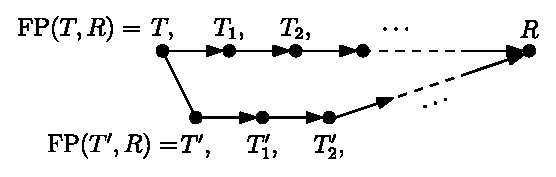
\includegraphics[width=0.6\textwidth]{proof_idea_ag}
\caption{Trees $T$, $T'$, and $R$ as in inequality~(\ref{eqn:iff_inequality}).
Paths $\fp(T,R) = [T,T_1,T_2, \ldots, R]$ and $\fp(T',R) = [T',T'_1,T'_2, \ldots, R]$ are indicated by arrows.}
\label{fig:proof_idea}
\end{figure}

Assume to the contrary that $T$ and $R$ are trees for which there exists $T'$ violating inequality~(\ref{eqn:iff_inequality}).
Out of all such pairs $T, R$ choose one with the minimal $|\fp(T, R)|$.
Denote $\fp(T,R) = [T, T_1, T_2, \ldots, R]$ and $\fp(T', R) = [T', T_1', T_2', \ldots, R]$, and let $[(T)_t, (T)_{t+1}]$ be the interval in $T$ on which the $\rnni$ move connecting $T$ and $T'$ is performed.
Let $C_k$ be the cluster of $R$ such that the node $(C_k)_T$ is moved down by the first move on $\fp(T, R)$.
If the rank of $(C_k)_T$ is not in $\{t, t+1\}$ then $(C_k)_T$ and $(C_k)_{T'}$ induce the same cluster, so $\findpath$ would make the same rearrangement in both trees $T$ and $T'$ in the first move along $\fp(T, R)$ and $\fp(T', R)$ resulting in trees $T_1$ and $T_1'$ which are $\rnni$ neighbours, as in Figure~\ref{fig:proof_idea}.
In this case, paths $\fp(T_1, R)$ and $\fp(T_1', R)$ violate inequality~(\ref{eqn:iff_inequality}) but $\fp(T_1, R)$ is strictly shorter than $\fp(T, R)$, contradicting our minimality assumption.
Hence, the first move on $\fp(T, R)$ has to involve an interval incident to at least one of the nodes $(T)_t$, $(T)_{t+1}$.

We will distinguish two cases depending on whether $T$ and $T'$ are connected by an $\nni$ or a rank move.
For each of these we will further distinguish all possible moves between $T$ and $T_1$.
Note that in all figures illustrating possible moves on $\fp(T,R)$ and $\fp(T',R)$, the positions of tree roots are irrelevant, so we have positioned the roots to simplify our figures.

\textbf{Case 1.}
$T$ and $T'$ are connected by an $\nni$ move, so $((T)_t,(T)_{t+1})$ is an edge in $T$ -- see Figure~\ref{fig:thm_fp_nni1}.
Denote the clusters induced by the children of $(T)_t$ by $A$ and $B$ and the cluster induced by the child of $(T)_{t+1}$ that is not $(T)_t$ by $C$, and assume that the $\nni$ move between $T$ and $T'$ exchanges the subtrees induced by clusters $B$ and $C$.
Additionally, denote the cluster induced by the child of $(T)_{t+2}$ that is not $(T)_{t+1}$ by $D$ -- see Figure~\ref{fig:thm_fp_nni2a}.

\begin{figure}[!hbt]
\centering
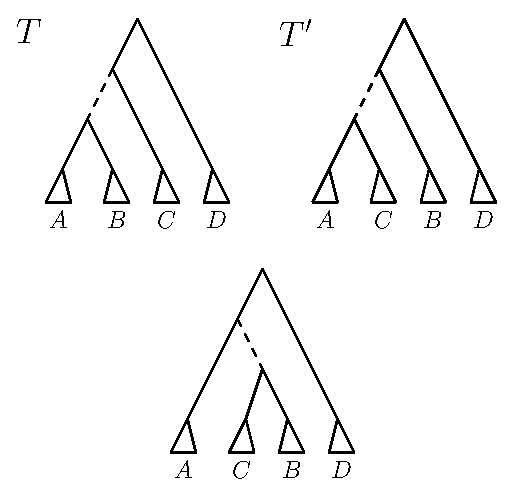
\includegraphics[width=0.35\textwidth]{thm_fp_nni1}
\caption{$\nni$ move between $T$ and $T'$ on the bold edge $((T)_t,(T)_{t+1})$ and the third $\rnni$ neighbour resulting from a move on that edge.}
\label{fig:thm_fp_nni1}
\end{figure}

We now consider all possible moves $\findpath$ can perform to go from $T$ to $T_1$ that involve a node of rank $t$ or $t+1$, that is, we will consider three intervals in total.

\begin{enumerate}[label = 1.{\arabic*}]
\item $\rnni$ move on interval $[(T)_t, (T)_{t+1}]$.
Note that this move has to be the $\nni$ move that is different from the $\nni$ move connecting $T$ and $T'$.

In this case, the cluster $B \cup C$ is built in $T_1$, as depicted in the bottom of Figure~\ref{fig:thm_fp_nni1}.
It follows that the cluster $C_k$ that is considered first by $\findpath$ must contain elements from both $B$ and $C$.
But then $\findpath$ applied to $T'$ and $R$ has to decrease the rank of $(C_k)_{T'}$ in its first step implying that $T'_1 = T_1$, so $|\fp(T',R)| = |\fp(T,R)|$.
This contradicts our assumption that $|\fp(T',R)| < |\fp(T,R)| - 1$.

\item $\nni$ move on (edge) interval $[(T)_{t+1}, (T)_{t+2}]$ that swaps the subtrees induced by clusters $C$ and $D$.
This move is shown in Figure~\ref{fig:thm_fp_nni2a} by an arrow from $T$ to the leftmost tree in the middle row.

\begin{figure}[H]
	\begin{subfigure}[b]{.45\textwidth}
		\centering
		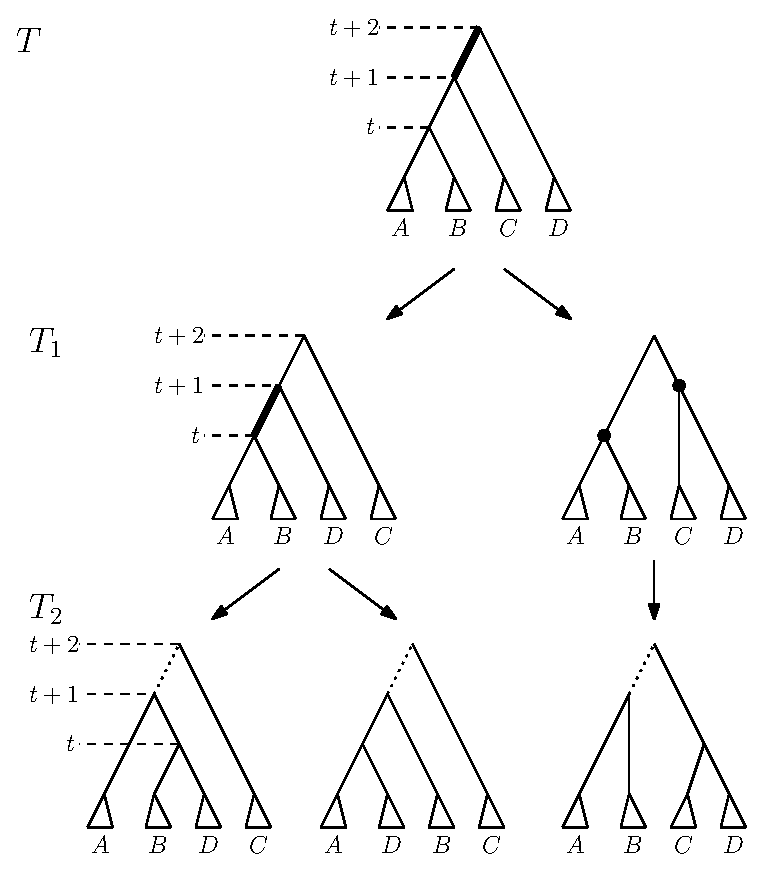
\includegraphics[width=0.9\linewidth]{thm_fp_nni2a.eps}
		\vspace{12pt}
		\caption{Possible initial segments of $\fp(T, R)$}
		\label{fig:thm_fp_nni2a}
	\end{subfigure}
	\begin{subfigure}[b]{.45\textwidth}
		\centering
		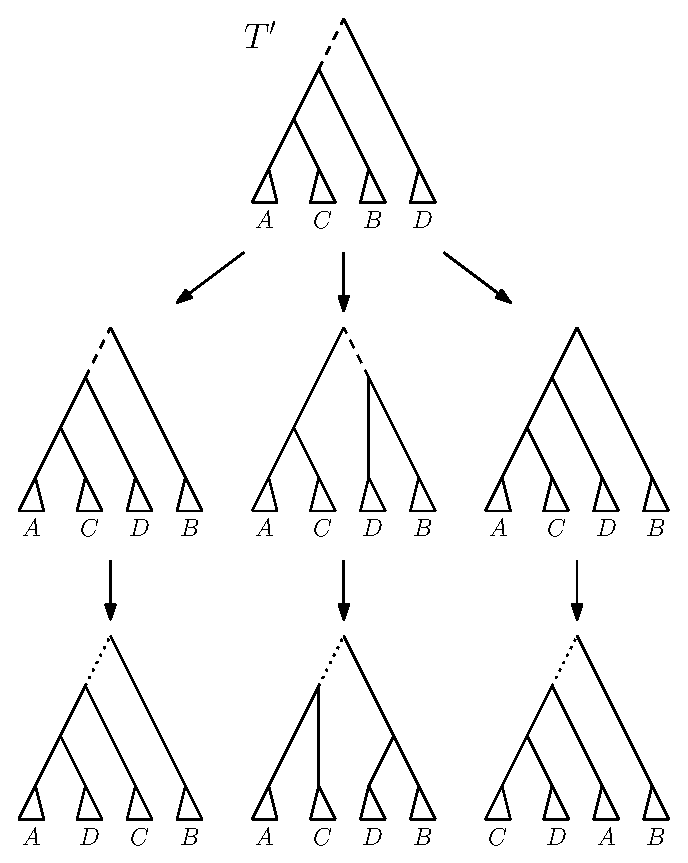
\includegraphics[width=0.9\linewidth]{thm_fp_nni2b.eps}
		\vspace{12pt}
		\caption{Possible initial segments of $\fp(T', R)$}
		\label{fig:thm_fp_nni2b}
	\end{subfigure}
	\caption{Comparison of paths $\fp(T, R)$ and $\fp(T', R)$ if $T$ and $T'$ are connected by an $\nni$ move on edge $((T)_{t+1},T_{t+2})$ in $T$.
	The bottom row displays all possibilities for $T_2$ and $T'_2$, depending on the position of cluster $C_k$ that is considered by $\findpath$:
	${C_k \subseteq B \cup D}$ is on the left, ${C_k \subseteq A \cup D}$ is in the middle, ${C_k \subseteq C \cup D}$ is on the right.}
	\label{fig:thm_fp_nni}
\end{figure}

Note that the cluster $C_k$ that is considered by $\findpath$ in the first step of computing $\fp(T, R)$ must intersect $D$.
Additionally, $C_k$ must intersect $A$, or $B$, or both of them.
Hence, we will consider each of these three cases individually.

We will use Figure~\ref{fig:thm_fp_nni} to demonstrate all the three cases below.

\begin{enumerate}[label = \theenumi.\arabic*]
\item $C_k$ intersects each of $A$, $B$, and $D$.
We can assume $k > 1$ and $C_{k-1} = (R)_{k-1}$ as $C_1$ contains two elements and can therefore only intersect with either $A$ or $B$.
Since $C_k$ is the first cluster considered by $\findpath$, the two clusters that make up $C_k$ in $R$ must be present in $T$.
So $C_{k-1} = A \cup B$.
Since $A \cup B$ is not a cluster in $T'$, $\findpath$ will decrease the rank of $(C_{k-1})_{T'}$ on $\fp(T', R)$ before considering cluster $C_k$.
Note that the clusters induced by nodes of rank $i < k - 1$ in $T$ and $T'$ coincide, so all moves, if any, on $\fp(T, R)$ and $\fp(T', R)$ that involve those cluster will be the same.
The $\rnni$ move decreases the rank of $(C_{k-1})_{T'}$ by building cluster $A \cup B$, in which case $T'_1 = T$.
This however contradicts $|\fp(T',R)| < |\fp(T,R)| - 1$.

\item $C_k \subseteq A \cup D$.
\label{deep_case_details}
Starting from $T$, $\findpath$ exchanges first subtrees induced by clusters $C$ and $D$ and then by $B$ and $D$.
This results in trees $T_1$ and $T_2$ -- see the path leading to the tree in the middle of the bottom row in Figure~\ref{fig:thm_fp_nni2a}.
Starting from $T'$, $\findpath$ exchanges first subtrees induced by $B$ and $D$ and then by $C$ and $D$.
This results in trees $T_1'$ and $T_2'$ -- see the path leading to the tree in the middle of the bottom row in Figure~\ref{fig:thm_fp_nni2b}.
It follows that $T_2$ and $T'_2$ only differ by one interval (indicated by dotted edges in the corresponding trees in Figure~\ref{fig:thm_fp_nni}), and hence they are $\rnni$ neighbours.
This together with the facts that $|\fp(T_2,R)| = |\fp(T,R)|-2$ and $|\fp(T'_2,R)| = |\fp(T',R)|-2$ contradicts the assumption that $|\fp(T,R)|$ is a minimal length violating inequality~(\ref{eqn:iff_inequality}).

\item $C_k \subseteq B \cup D$.
This case is analogous to the previous one.
The two initial segments of $\fp(T, R)$ and $\fp(T', R)$ are the paths leading to the leftmost trees in the bottom row of Figures~\ref{fig:thm_fp_nni2a} and \ref{fig:thm_fp_nni2b}, respectively.
Note that the rank swap leading from $T_1'$ to $T_2'$ is required because the rank of $(C_k)_R$ is at most $t$ as implied by the move leading from $T_1$ to $T_2$.
The corresponding trees $T_2$ and $T_2'$ are again $\rnni$ neighbours.
\end{enumerate}

\item $\nni$ move on (edge) interval $[(T)_{t+1}, (T)_{t+2}]$ that builds a cluster $C \cup D$ in $T_1$.
\label{case:one_or_two_moves_down}
This move is shown in Figure~\ref{fig:thm_fp_nni2a} by an arrow from $T$ to the second leftmost tree in the middle row.
In this case, $C_k \subseteq C \cup D$.

If the ranks of $(C_k)_{T_1}$ and $(C_k)_R$ coincide then $C_{k-1} = A \cup B$ is a cluster in $R$.
Since $A \cup B$ is not a cluster in $T'$, the first $\rnni$ move on $\fp(T', R)$ builds the cluster $A \cup B$ by swapping subtrees induced by cluster $B$ and $C$.
This move results in $T_1' = T$ contradicting $|\fp(T',R)| < |\fp(T,R)| - 1$.

If the rank of $(C_k)_{T_1}$ is strictly higher than that of $(C_k)_R$ then $\findpath$ decreases the rank of $(C_k)_{T_1}$ in the second step.
This results in the path from $T$ to the rightmost tree in Figure~\ref{fig:thm_fp_nni2a}.
Hence, $\fp(T', R)$ also has to begin with two moves that decrease the rank of $(C_k)_{T'}$ twice, resulting in the rightmost path in Figure~\ref{fig:thm_fp_nni2b}.
Similarly to case~\ref{deep_case_details}, we arrive at a contradiction that trees $T_2$, $T_2'$, and $R$ violate inequality~(\ref{eqn:iff_inequality}) and $|\fp(T_2,R)| < |\fp(T,R)|$.

\item Rank move on interval $[(T)_{t+1},(T)_{t+2}]$.
\label{case:rank_move_interval_above}
This case is analogous to case~\ref{case:one_or_two_moves_down}.
If the ranks of $(C_k)_{T_1}$ and $(C_k)_R$ coincide then $C_{k-1} = A \cup B$ is a cluster in $R$, and applying $\findpath$ to $T', R$ we get $T'_1 = T$.
If the rank of $(C_k)_{T_1}$ is strictly higher than that of $(C_k)_R$ then $\findpath$ decreases the rank of $(C_k)_{T_1}$ in the second step.
Recall that the interval between nodes of rank $t$ and $t+1$ is an edge in both $T$ and $T'$.
Hence, the first two moves on $\fp(T', R)$ decrease the rank of $(C_k)_{T'}$ twice resulting in $T'_2$ which is an $\rnni$ neighbour of $T_2$.
As before, this contradicts our minimality assumption.

\item $\rnni$ move on interval $[(T)_{t-1},(T)_t]$.
In this case $C_k \subseteq A \cup B$, so the first move on $\fp(T', R)$ decreases the rank of $(C_k)_{T'}$ by exchanging the subtrees induced by $B$ and $C$.
This results in $T'_1 = T$.
This argument applies whether or not $((T)_{t-1},(T)_t)$ is an edge in $T$.
\end{enumerate}

\textbf{Case 2.}
$T$ and $T'$ are connected by a rank move on the interval between nodes of rank $t$ and $t+1$.
Denote the cluster induced by $(T)_t$ by $A$, the clusters induced by the children of $(T)_t$ by $A_1$ and $A_2$, the cluster induced by $(T)_{t+1}$ by $B$, and the clusters induced by the children of $(T)_{t+1}$ by $B_1$ and $B_2$ -- see Figure~\ref{fig:thm_fp_rank1}.

\begin{figure}[!hbt]
\centering
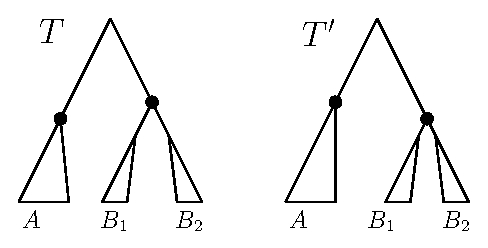
\includegraphics[width=0.4\textwidth]{thm_fp_rank1}
\caption{Rank move between $T$ and $T'$ on the interval above the node of rank $t$, and possible initial segments of $\fp(T, R)$ and $\fp(T', R)$.
We use notations $A = A_1 \cup A_2$ and $B = B_1 \cup B_2$.}
\label{fig:thm_fp_rank1}
\end{figure}

We again consider all possible moves $\findpath$ can perform to go from $T$ to $T_1$ that involve a node of rank $t$ or $t+1$.

\begin{enumerate}[label = 2.\arabic*]
\item Rank move on $[(T)_t,(T)_{t+1}]$.
This move results in $T_1 = T'$.

\item $\nni$ move on (edge) interval $[(T)_{t+1},(T)_{t+2}]$.
The following two sub-cases are analogous to case~\ref{case:one_or_two_moves_down}.

\begin{enumerate}[label = \theenumi.\arabic*]
	\item $(T)_{t+2}$ is a parent of $(T)_t$.
	The first move on $\fp(T, R)$ builds a cluster $A \cup B_1$ or $A \cup B_2$, and we assume without loss of generality that it is the former, as in Figure~\ref{fig:thm_fp_rank1}.
	This implies that $C_k \subseteq A \cup B_1$.
	If the ranks of $(C_k)_{T_1}$ and $(C_k)_R$ coincide then $C_{k-1} = A$ is a cluster in $R$.
	Therefore, the first move on $\fp(T', R)$ decreases the rank of $(A)_{T'}$, which results in $T_1' = T$.
	If the rank of $(C_k)_{T_1}$ is strictly higher than that of $(C_k)_R$ then $\findpath$ decreases the rank of $(C_k)_{T_1}$ in the second step.
	Due to the symmetry we can assume that $C_k \subseteq A_1 \cup B_1$, which implies that the move between $T_1$ to $T_2$ exchanges the subtrees induced by $A_2$ and $B_1$, as depicted on the left of Figure~\ref{fig:thm_fp_rank1}.
	$C_k \subseteq A_1 \cup B_1$ implies that the first two moves on $\fp(T', R)$ result in a tree $T'_2$ that is an $\rnni$ neighbour of $T_2$ -- see Figure~\ref{fig:thm_fp_rank1}.
	This is a contradiction to the minimality assumption on $|\fp(T,R)|$.

	\item $(T)_{t+2}$ is not a parent of $(T)_t$.
	In this case, there exists a cluster $C$ induced by the child of $(T)_{t+2}$ which is different from the one that induces $B$ -- see Figure~\ref{fig:thm_fp_rank2}.
\begin{figure}[!hbt]
	\centering
	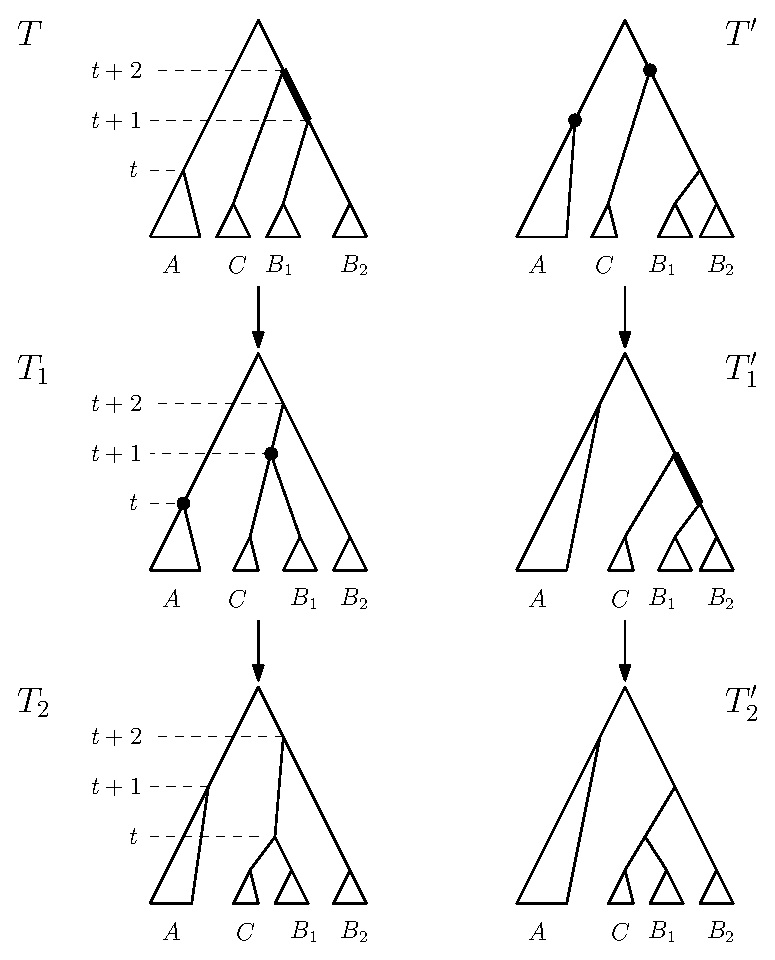
\includegraphics[width=0.4\textwidth]{thm_fp_rank2}
	\caption{Comparison of paths $\fp(T, R)$ and $\fp(T', R)$ if there is a rank move between $T$ and $T'$ and an $\nni$ move on the edge below the corresponding (rank) interval follows on $\fp(T, R)$.}
	\label{fig:thm_fp_rank2}
\end{figure}
	We can assume without loss of generality that $C_k \subseteq C \cup B_1$ and the first move on $\fp(T, R)$ builds a new cluster $C \cup B_1$.
	If the ranks of $(C_k)_{T_1}$ and $(C_k)_R$ coincide then $C_{k-1} = A$ is a cluster in $R$, which implies that $A$ is induced by the node of rank $t$ in both $T$ and $R$.
	So $T'_1 = T$.
	If the rank of $(C_k)_{T_1}$ is strictly higher than that of $(C_k)_R$ then $\findpath$ decreases the rank of $(C_k)_{T_1}$ in the second step -- see Figure~\ref{fig:thm_fp_rank2}.
	The corresponding first moves on $\fp(T', R)$ are shown on the right in Figure~\ref{fig:thm_fp_rank2}, and we again get that $T_2$ and $T_2'$ are $\rnni$ neighbours.
\end{enumerate}

\item Rank move on interval $[(T)_{t+1}, (T)_{t+2}]$.
Again, depending on whether or not the ranks of $(C_k)_{T_1}$ and $(C_k)_R$ coincide, we arrive at the conclusion that either $T_1' = T$ or $T_2$ and $T_2'$ are $\rnni$ neighbours, similar to case~\ref{case:rank_move_interval_above}.

\item $\rnni$ move on interval $[(T)_{t-1},(T)_t]$.
In this case $C_k \subseteq A$ and the first move on $\fp(T', R)$ must be a rank swap resulting in $T_1' = T$.
\end{enumerate}

Since all possible cases result in a contradiction, we conclude that inequality~(\ref{eqn:iff_inequality}) is true for all trees, which completes the proof of the theorem.
\endproof

\summary{Proving the Cluster Property for $\rnni$}

\begin{corollary}
	Let $T$ and $R$ be two trees sharing a cluster $C$ and $p$ a shortest path from $T$ to $R$ in $\rnni$.
	Then every tree on $p$ contains the cluster $C$.
	\label{cluster_thm}
\end{corollary}

\proof
	Assume to the contrary that $T$, $R$, $C$, and $p$ is a courter-example to the statement.
	We can assume that no counterexample exists for paths shorter than $p$, so the first tree $T'$ after $T$ on $p$ does not contain the cluster $C$.
	Therefore $T$ and $T'$ are connected by an $\nni$ move that moves a subtrees rooted at a child of $(C)_T$ out of the subtree induced by $C$ -- see Figure~\ref{fig:cluster_thm_proof}, where by $C_1$, $C_2$ we denote the clusters induced by the children of $(C)_T$.
	Note that the only clusters in $T$ that distinguish $T$ from $T'$ are $C$ and the cluster induced by the node right above $(C)_{T}$, which is of the same rank as $(C)_{T'}$.

	\begin{figure}[!hbt]
	\centering
	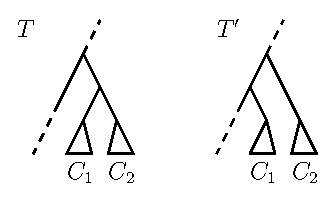
\includegraphics[width=0.3\textwidth]{cluster_thm_proof}
	\caption{Neighbouring trees $T$ and $T'$, where $T$ contains the cluster $C = C_1 \cup C_2$ and $T'$ does not.
	Dashed lines indicate identical trees.}
	\label{fig:cluster_thm_proof}
	\end{figure}

	Since $T$ and $R$ have the minimum possible distance among all counterexamples to the theorem, we can assume, using the same argument as in the beginning of the proof of Theorem~\ref{thm:rnni_polynomial}, that $C$ is the first cluster considered by $\findpath$ on $\fp(T, R)$.
	But in this case, the first move on $\fp(T',R)$ builds the cluster $C$ and results in tree $T$, which is a contradiction.
\endproof


\section{Generalisation to discrete time-trees}

\summary{Generalising} $\findpath$ \summary{for discrete time-trees}
We now consider the obvious extension of $\findpath$ to discrete time-trees.

\begin{corollary}
	$\findpath$ computes shortest paths between discrete time-trees.
\end{corollary}

\proof
	Let $T$ and $R$ be discrete time-trees and let $m$ be the maximum of the times assigned to the roots of $T$ and $R$.
	We construct trees $T'$ and $R'$ in $\rnni$ on $m + 1$ leaves by adding $m + 1 - n$ new leaves in the following way.
	Add a new root with rank $m+1$ to tree $T$, such that $T$ is a subtree rooted in one of the children of this new node.
	The other child of this new root is a caterpillar tree with leaf labels in $\{n+1, \ldots, m+1\}$ such that the ranks of the parents of these leaves are ordered according to the leaf labels and the resulting tree does not contain intervals of length greater than one.
	The same way we obtain tree $R'$ from $R$.

	We can convert a path $p$ from $T$ to $R$ to a path $p'$ from $T'$ to $R'$ so that $|p| = |p'|$ by exchanging all length moves on $p$ to rank swaps on $p'$.
	All rank moves and $\nni$ moves on $p'$ remain the same as on $p'$.
	By the construction of $T'$ and $R'$ it follows that $p'$ ends in $R'$, as the additional caterpillar subtree does not change.
	As every move on $p$ corresponds to exactly one move on $p'$, the lengths of these paths coincide.

	$\fp(T,R)$ is defined by transforming the moves along $\fp(T',R')$ in the similar way.
	To show that $\fp(T, R)$ computes a shortest path, we observe that if there was another path $p$ from $T$ to $R$ strictly shorter than $\fp(T, R)$, we can construct a path $p'$ with $|p'| = |p| < |\fp(T,R)| = |\fp(T',R')s|$ between $T'$ and $R'$ as explained above, which is a contradiction to Theorem~\ref{thm:rnni_polynomial}.
\endproof

\summary{Why the complexity of $\rnni(\rho)$ might be different from $\nni$ or $\rnni$ for $\rho$ big enough.}


\section{Conclusion}

\summary{Useful observation for rounding up the discussion about $\rnni(\rho)$ -- should be put where we do that.}
When considering the problem of characterising the complexity of computing the distance in $\rnni(\rho)$, an important question is how to balance the trade off between $\nni$ and rank moves.
Indeed, examples exist when different shortest paths between trees have different number of $\nni$ moves, that is, some $\nni$ moves can be traded for rank moves.
The following observation, which directly follows from Theorem~\ref{thm:rnni_polynomial}, provides a first step towards understanding of this trade off using the $\findpath$ algorithm.

\begin{corollary}
	For every pair of discrete time-trees $T$ and $R$, $\fp(T, R)$ has the minimal possible number of moves changing the ranked topology, among all shortest paths between $T$ and $R$.
	\label{prpn:FP_minimises_topology_changes}
\end{corollary}

As we have shown, the complexity of computing the nearest neighbour interchange distance between ranked phylogenetic trees depends on the weight of rank rearrangements and can change from quadratic, when rank moves are counted as one rearrangement, to NP-hard, when rank moves are ignored.
It hence is natural to ask whether a boundary exists at which the problem switches from polynomial to hard.
In what follows we consider this question in more detail and leave its complete solution as an open problem.

\newpage


\printbibliography
\end{document}
